
	\section{ACM/ICPC World Finals 2004}
		\subsection{ACM/ICPC World Finals 2004 A Carl the Ant}
			\subsubsection{题目大意}
				有若干只蚂蚁从地下穿到地面,行走一段距离后,穿回洞穴。
				
				蚂蚁以相同时间间隔 $d$ 出洞。
				
				有一只蚂蚁在最前面带路,且在路上的行走过程中都沿着每格为单位长度的网格格线走(起点和终点位于网格格点)。其他蚂蚁则跟着带队的蚂蚁留下的气味走。
				
				每支蚂蚁长度均为单位长度,速度均为单位速度,且会沿着带队的蚂蚁\emph{最新}留下的气味走。
				
				如果两只蚂蚁接下来会碰撞,那么\emph{等待了最久的蚂蚁先走},而如果两只蚂蚁等待的时间相同,那么\emph{走了最远路径的先走},另一只蚂蚁则停下。若有蚂蚁在洞口附近停下并堵住洞口,那么洞口的蚂蚁也会排好队,等会依次通过。
				
				问全部蚂蚁回到洞穴的时间及其先后顺序。
				
				带头蚂蚁在路上行走的长度 $N\le 50$,蚂蚁总数 $M \le 100$。$1 \le d \le 100$。
			\subsubsection{算法讨论}
				由于所有的蚂蚁都在网格线上运动,那么使用一个二维数组模拟它们的运动就可以了。二维数组的尺寸 $(2N + 1) \times (2N + 1)$。
				
				需要细心地处理两只蚂蚁将要碰撞时,谁走先谁走后的问题。
%				为了模拟的方便,可在之前对蚂蚁的优先级拍个序,模拟时按照顺序运动。
				模拟时可能需要用到类似 Bellman-Ford 的算法,因为不便于确定移动各个蚂蚁的先后顺序。
				
				按照模拟的结果输出答案。
			\subsubsection{时空复杂度}
				时间复杂度 $\mathcal{O}\left(N^2 + N \cdot \min(M,d)\cdot M k\right)$。 $k$ 是 Bellman-Ford 算法迭代的次数,实践起来此值较小。
					
				空间复杂度 $\mathcal{O}\left(N^2\right)$。


		\newpage
		\subsection{ACM/ICPC World Finals 2004 B Heliport}
			\subsubsection{题目大意}
				如图 \ref{2004b} 中的两例,给出一个正交的简单多边形,求最大的内接圆半径。
				
									\begin{figure}[htb]
\centering
\begin{minipage}{.6\textwidth}
  \centering

\definecolor{ffccww}{rgb}{1,0.8,0.4}
\definecolor{cczzqq}{rgb}{0.8,0.6,0}
\definecolor{cqcqcq}{rgb}{0.75,0.75,0.75}
\begin{tikzpicture}[line cap=round,line join=round,>=stealth',x=1.0cm,y=1.0cm,scale = 0.8]
\draw [color=cqcqcq,dash pattern=on 2pt off 2pt, xstep=1.0cm,ystep=1.0cm] (0,0) grid (7.5,5.5);
\draw[->,color=black] (-0.4,0) -- (7.92,0) node[right] {$x$};
\foreach \x in {,1,2,3,4,5,6,7}
\draw[shift={(\x,0)},color=black] (0pt,2pt) -- (0pt,-2pt) node[below] {\footnotesize $\x$};
\draw[->,color=black] (0,-0.42) -- (0,5.82) node[left] {$y$};
\foreach \y in {,1,2,3,4,5}
\draw[shift={(0,\y)},color=black] (2pt,0pt) -- (-2pt,0pt) node[left] {\footnotesize $\y$};
\draw[color=black] (0pt,-10pt) node[left] {\footnotesize $0$};
\clip(-0.47,-0.42) rectangle (7.92,5.82);
\fill[color=ffccww,fill=ffccww,fill opacity=0.2] (1,5) -- (6,5) -- (6,4) -- (5,4) -- (5,2) -- (7,2) -- (7,1) -- (4,1) -- (4,2) -- (3,2) -- (3,1) -- (1,1) -- (1,2) -- (2,2) -- (2,3) -- (1,3) -- cycle;
\draw [color=ffccww] (1,5)-- (6,5);
\draw [color=ffccww] (6,5)-- (6,4);
\draw [color=ffccww] (6,4)-- (5,4);
\draw [color=ffccww] (5,4)-- (5,2);
\draw [color=ffccww] (5,2)-- (7,2);
\draw [color=ffccww] (7,2)-- (7,1);
\draw [color=ffccww] (7,1)-- (4,1);
\draw [color=ffccww] (4,1)-- (4,2);
\draw [color=ffccww] (4,2)-- (3,2);
\draw [color=ffccww] (3,2)-- (3,1);
\draw [color=ffccww] (3,1)-- (1,1);
\draw [color=ffccww] (1,1)-- (1,2);
\draw [color=ffccww] (1,2)-- (2,2);
\draw [color=ffccww] (2,2)-- (2,3);
\draw [color=ffccww] (2,3)-- (1,3);
\draw [color=ffccww] (1,3)-- (1,5);
\draw(3.5,3.5) circle (1.5cm);
\begin{scriptsize}
\fill [color=cczzqq] (1,5) circle (1.5pt);
\draw[color=cczzqq] (1.1,5.22) node {$A$};
\fill [color=cczzqq] (6,5) circle (1.5pt);
\draw[color=cczzqq] (6.12,5.22) node {$B$};
\fill [color=cczzqq] (6,4) circle (1.5pt);
\draw[color=cczzqq] (6.12,4.24) node {$C$};
\fill [color=cczzqq] (5,4) circle (1.5pt);
\draw[color=cczzqq] (5.12,4.24) node {$D$};
\fill [color=cczzqq] (5,2) circle (1.5pt);
\draw[color=cczzqq] (5.12,2.23) node {$E$};
\fill [color=cczzqq] (7,2) circle (1.5pt);
\draw[color=cczzqq] (7.11,2.23) node {$F$};
\fill [color=cczzqq] (7,1) circle (1.5pt);
\draw[color=cczzqq] (7.12,1.22) node {$G$};
\fill [color=cczzqq] (4,1) circle (1.5pt);
\draw[color=cczzqq] (4.13,1.22) node {$H$};
\fill [color=cczzqq] (4,2) circle (1.5pt);
\draw[color=cczzqq] (4.08,2.23) node {$I$};
\fill [color=cczzqq] (3,2) circle (1.5pt);
\draw[color=cczzqq] (3.11,2.23) node {$J$};
\fill [color=cczzqq] (3,1) circle (1.5pt);
\draw[color=cczzqq] (3.12,1.22) node {$K$};
\fill [color=cczzqq] (1,1) circle (1.5pt);
\draw[color=cczzqq] (1.1,1.22) node {$L$};
\fill [color=cczzqq] (1,2) circle (1.5pt);
\draw[color=cczzqq] (1.12,2.23) node {$M$};
\fill [color=cczzqq] (2,2) circle (1.5pt);
\draw[color=cczzqq] (2.12,2.23) node {$N$};
\fill [color=cczzqq] (2,3) circle (1.5pt);
\draw[color=cczzqq] (2.12,3.23) node {$O$};
\fill [color=cczzqq] (1,3) circle (1.5pt);
\draw[color=cczzqq] (1.12,3.23) node {$P$};
\end{scriptsize}
\end{tikzpicture}
\end{minipage}%
\begin{minipage}{.4\textwidth}
  \centering
\definecolor{ffccww}{rgb}{1,0.8,0.4}
\definecolor{cczzqq}{rgb}{0.8,0.6,0}
\definecolor{cqcqcq}{rgb}{0.75,0.75,0.75}
\begin{tikzpicture}[line cap=round,line join=round,>=stealth',x=1.0cm,y=1.0cm,scale = 0.8]
\draw [color=cqcqcq,dash pattern=on 2pt off 2pt, xstep=1.0cm,ystep=1.0cm] (-0,0) grid (5.2,5.5);
\draw[->,color=black] (-0.4,0) -- (5.68,0) node[right] {$x$};
\foreach \x in {,1,2,3,4,5}
\draw[shift={(\x,0)},color=black] (0pt,2pt) -- (0pt,-2pt) node[below] {\footnotesize $\x$};
\draw[->,color=black] (0,-0.42) -- (0,5.82) node[left] {$y$};
\foreach \y in {,1,2,3,4,5}
\draw[shift={(0,\y)},color=black] (2pt,0pt) -- (-2pt,0pt) node[left] {\footnotesize $\y$};
\draw[color=black] (0pt,-10pt) node[left] {\footnotesize $0$};
\clip(-0.4,-0.43) rectangle (5.68,5.61);
\fill[color=ffccww,fill=ffccww,fill opacity=0.2] (1,5) -- (5,5) -- (5,2) -- (4,2) -- (4,1) -- (1,1) -- cycle;
\draw [color=ffccww] (1,5)-- (5,5);
\draw [color=ffccww] (5,5)-- (5,2);
\draw [color=ffccww] (5,2)-- (4,2);
\draw [color=ffccww] (4,2)-- (4,1);
\draw [color=ffccww] (4,1)-- (1,1);
\draw [color=ffccww] (1,1)-- (1,5);
\draw(2.76,3.24) circle (1.76cm);
\begin{scriptsize}
\fill [color=cczzqq] (1,5) circle (1.5pt);
\draw[color=cczzqq] (1.1,5.21) node {$A$};
\fill [color=cczzqq] (5,5) circle (1.5pt);
\draw[color=cczzqq] (5.12,5.21) node {$B$};
\fill [color=cczzqq] (5,2) circle (1.5pt);
\draw[color=cczzqq] (5.12,2.22) node {$C$};
\fill [color=cczzqq] (4,2) circle (1.5pt);
\draw[color=cczzqq] (4.12,2.22) node {$D$};
\fill [color=cczzqq] (4,1) circle (1.5pt);
\draw[color=cczzqq] (4.12,1.22) node {$E$};
\fill [color=cczzqq] (1,1) circle (1.5pt);
\draw[color=cczzqq] (1.1,1.22) node {$F$};
\end{scriptsize}
\end{tikzpicture}




\end{minipage}
  \caption{}
  \label{2004b}
\end{figure}
				
				多边形点数 $N \le 20$,保证边与坐标轴平行或垂直。
			\subsubsection{算法讨论}
				我们可以给出一个求任意简单多边形(不要求边正交,即与坐标轴平行或垂直)的最大内接圆半径的算法。算法的核心在于说明,肯定存在一个最优的内接圆,与多边形边界交于至少三点。


									\begin{figure}[b]
\centering
\begin{minipage}{.3\textwidth}
  \centering

\definecolor{qqwuqq}{rgb}{0,0.39,0}
\definecolor{qqqqff}{rgb}{0,0,1}
\begin{tikzpicture}[line cap=round,line join=round,>=triangle 45,x=1.0cm,y=1.0cm]
\clip(-0.55,0.24) rectangle (4.95,5.17);
\draw [shift={(3,3)},color=qqwuqq,fill=qqwuqq,fill opacity=0.1] (0,0) -- (90:0.36) arc (90:270:0.36) -- cycle;
\draw [dash pattern=on 3pt off 3pt] (3,0.24) -- (3,5.17);
\draw [domain=-0.5507425556704313:3.0] plot(\x,{(-18--5*\x)/-1});
\draw [domain=-0.5507425556704313:3.0] plot(\x,{(-12--2*\x)/-2});
\draw [domain=-0.5507425556704313:3.0] plot(\x,{(-6-0*\x)/-2});
\draw [domain=-0.5507425556704313:3.0] plot(\x,{(-0-2*\x)/-2});
\draw [domain=-0.5507425556704313:3.0] plot(\x,{(--6-3*\x)/-1});
% \draw [dash pattern=on 3pt off 3pt] (3,-3) -- (3,0.24);
\begin{scriptsize}
\fill [color=qqqqff] (3,3) circle (1.5pt);
\fill [color=qqqqff] (0,3) circle (1.5pt);
\draw[color=qqwuqq] (3.58,3.05) node {$\alpha = \pi$};
\end{scriptsize}
\end{tikzpicture}

  \caption{}
  \label{2004b2}


\end{minipage}%
\begin{minipage}{.4\textwidth}
  \centering
\definecolor{cczzqq}{rgb}{0.8,0.6,0}
\definecolor{ffccww}{rgb}{1,0.8,0.4}
\definecolor{ttffqq}{rgb}{0.2,1,0}
\definecolor{ttzzqq}{rgb}{0.2,0.6,0}
\begin{tikzpicture}[line cap=round,line join=round,>=triangle 45,x=1.0cm,y=1.0cm, scale = 0.65]
\clip(-3.45,-2.26) rectangle (5.36,5.36);
\fill[color=ttffqq,fill=ttffqq,fill opacity=0.1] (-1,3) -- (0,5) -- (2,5) -- (3,3) -- (5,2) -- (4,-2) -- (-2,-2) -- (-3,2) -- cycle;
\draw [color=ttffqq] (-1,3)-- (0,5);
\draw [color=ttffqq] (0,5)-- (2,5);
\draw [color=ttffqq] (2,5)-- (3,3);
\draw [color=ttffqq] (3,3)-- (5,2);
\draw [color=ttffqq] (5,2)-- (4,-2);
\draw [color=ttffqq] (4,-2)-- (-2,-2);
\draw [color=ttffqq] (-2,-2)-- (-3,2);
\draw [color=ttffqq] (-3,2)-- (-1,3);
\draw [line width=2pt,color=ffccww] (1,1.51) circle (2.49cm);
\draw [line width=2pt,color=cczzqq] (1,1.1) circle (2.76cm);
\begin{scriptsize}
\fill [color=ttzzqq] (-1,3) circle (1.5pt);
\draw[color=ttzzqq] (-0.8,3.43 - 1) node {};
\fill [color=ttzzqq] (3,3) circle (1.5pt);
\draw[color=ttzzqq] (3.23,3.43) node {};
\fill [color=ttzzqq] (1,1.51 - 1) circle (1.5pt);
\draw[color=ttzzqq] (1.21,1.94 - 0.8) node {$P$};
\fill [color=ttzzqq] (1,1.1) circle (1.5pt);
\draw[color=ttzzqq] (1.24,1.53 - 1) node {$P^\prime$};
\end{scriptsize}
\end{tikzpicture}

  \caption{}
  \label{2004b3}
\end{minipage}%
\begin{minipage}{.3\textwidth}
  \centering
\definecolor{qqzzcc}{rgb}{0,0.6,0.8}
\definecolor{ffzzzz}{rgb}{1,0.6,0.6}
\definecolor{zzttqq}{rgb}{0.6,0.2,0}
\begin{tikzpicture}[line cap=round,line join=round,>=triangle 45,x=1.0cm,y=1.0cm]
\clip(-2.42,2.56) rectangle (1.28,4.38);
\fill[color=zzttqq,fill=zzttqq,fill opacity=0.1] (-2,4) -- (1,4) -- (1,3) -- (-2,3) -- cycle;
\draw [color=zzttqq] (-2,4)-- (1,4);
\draw [color=zzttqq] (1,4)-- (1,3);
\draw [color=zzttqq] (1,3)-- (-2,3);
\draw [color=zzttqq] (-2,3)-- (-2,4);
\draw [line width=1.5pt,color=qqzzcc] (-1.5,3.5) circle (0.5cm);
\draw [line width=1.5pt,color=qqzzcc!70!white] (0,3.5) circle (0.5cm);
\begin{scriptsize}
\fill [color=ffzzzz] (-1.5,3.5) circle (1.5pt);
\draw[color=ffzzzz] (-1.35-0.15,3.78) node {$P^\prime$};
\fill [color=ffzzzz] (0,3.5) circle (1.5pt);
\draw[color=ffzzzz] (0.16-0.15,3.78) node {$P$};
\end{scriptsize}
\end{tikzpicture}
  \caption{}
  \label{2004b4}
\end{minipage}
\end{figure}


				{\theorem 存在一个最优的内接圆,与多边形边界交于至少三点。}
				\begin{pf}


					不妨假设其只交于两点,作出圆心,那么肯定存在一个方向,使得圆心向该方向运动后,不会更靠近两个点。因为如图 \ref{2004b2},如果圆心要靠近一个点,那么需要向长度为 $\pi$ 的一个开区间中的一个方向运动。两个这样的区间必然无法覆盖区间 $[0, 2\pi)$,随便选一个未被覆盖的角度,就是我们要找的方向。
					
					随后,只要将圆心向这个方向运动无穷小量,并在固定圆心之后,将半径取最大的可能值,就可以得到一个新解,且答案不会变差。例如图 
  \ref{2004b3},将圆心 $P$ 移动到 $P^\prime$。
					
					若继续移动,那么此圆总会碰到边界,与边界交于第三个点,例如 图 \ref{2004b4},将圆心 $P$ 移动到 $P^\prime$。而这样做答案不会更差
%					,
					。又初始解具有任意性,故根据调整法,此情况下命题得证。
					
					而若只有一个交点,或没有交点,
					证明
					同理
%					可证
					。\qed

				\end{pf}
				
				那么只要在多边形边界上枚举三点,求出一个最好的圆心就可以了。但是,多边形边界上的点有无穷多个。我们应分以下情况枚举交点(或交点
%				位于
				所在的边界),计算可能的最优圆心:
				\begin{enumerate}
					\item {\bf 三个交点均为多边形顶点}:直接求对应三角形的外心,具体地,求中垂线之交。
					\item{\bf  只有两个交点为多边形顶点}:此时圆过两定点,并与一条直线(第三点所在的边)相切。此时可求出两个顶点的中垂线,并以参数方程的形式,表示成点 $(a+b t, p + qt)$。求出其到此直线的距离 $d$。$d$ 应该与 $(a+b t, p + qt)$ 到两个顶点中任意一个的距离相同,以此建立方程,解参数 $t$,代回  $(a+b t, p + qt)$ 即为圆心。
					\item {\bf 只有一个交点为多边形顶点}:此时圆过一定点,并与两条直线相切。如果两线相交,此时可先作出两直线的角平分线(有两条,需分别考虑。),并同样地以参数方程 $(a+b t, p + qt)$ 表示。$(a+b t, p + qt)$  到 两线的距离与到 定点的距离应该相同,建立方程可解出  $t$,代回  $(a+b t, p + qt)$ 即为圆心。而若两线平行,那么作出到它们等距,且与它们平行的线,用同样的方法建立并解出方程,可求出圆心。
					\item {\bf 没有一个交点为多边形顶点}:那么需作出与三条直线均相切的圆,即求三角形内心。具体地,求出角平分线之交即可导出圆心。
				\end{enumerate}
				
				求到可能的圆心后,求出其到边界的最短距离。可以枚举多边形的边界,求点和\emph{线段}的距离,取最小值。此值就是该圆心对应的最大半径。
%				再
				求出所有圆心中,最大半径值最大的。这个值就是答案。
			\subsubsection{时空复杂度}
				时间复杂度 $\mathcal{O}\left(N^4\right)$。枚举点点点/点点边/点边边/边边边 $\mathcal{O}\left(N^3\right)$,再求圆心 $\mathcal{O}\left(1\right)$,再求最大半径 $\mathcal{O}\left(N\right)$。
					
				空间复杂度 $\mathcal{O}\left(N\right)$。\newpage
		\subsection{ACM/ICPC World Finals 2004 C Image Is Everything}
			\subsubsection{题目大意}
				一个 $N \times N \times N$ 的立体网格图形,每个格子里可能是一个有颜色的不透明立方块,或者什么都没有(透明)。
				
				给出它六个方向上的视图,问\emph{最多}有多少个格子里有立方块?
				
				保证有解。 $N \le 10$。
			\subsubsection{算法讨论}
				由于要最大化有立方块的格子,那么对于每个方向的视图,如果某一格有颜色,就要使得这一格上实际看到的立方快深度越浅越好(离观察者越近越好)。
				
				类似于 Bellman-Ford 的算法 \ref{2004c} 可以实现上述目标。
				\begin{algorithm}[H]
				\caption{}
				\label{2004c}
					\begin{algorithmic}[1]
						\State 图形 $F[\cdot][\cdot][\cdot] \gets \text{ 未知 }, OK \gets $ 真
						\For{$OK$}
							\State $OK \gets $ 假
							\For{枚举所有方向,以及该方向上视图的格子,记其颜色为 $c$}
								\For{深度 $d$。从 $d = 1$ 枚举到 $d = N$}
									\State 计算出该方向,该网格,该深度对应的三维坐标 $(x, y, z)$。
									\If{$c = \text{透明}$且 $F[x][y][z] \ne$ 透明}
										\State $F[x][y][z] \gets\text{透明} , OK \gets $ 真 \Comment{该格透明板上钉钉。}
									\EndIf
									\If{$c \ne\text{透明} $且 $(F[x][y][z] = \text{未知} \lor F[x][y][z] =  c)$ }
										\State $F[x][y][z] \gets c$,并跳出枚举 $d$ 的循环。
									\EndIf
%									\If{$c \ne\text{透明} $且 $F[x][y][z] = c$}
%										\State 跳出枚举 $d$ 的循环。
%									\EndIf
									\If{$c \ne \text{透明} $且 $F[x][y][z] \ne c$}
										\State $F[x][y][z] \gets\text{透明} , OK \gets $ 真 \Comment{产生矛盾
%										,只能改回透明
										}
									\EndIf
								\EndFor
							\EndFor
						\State 输出满足 $F[x][y][z] \ne \text{透明} $   的三元组数。 \Comment{$F[x][y][z]  = \text{未知}$ 的是无法被观察到的
%						格子
						}
						\EndFor
					\end{algorithmic}
				\end{algorithm}	
			\subsubsection{时空复杂度}
				时间复杂度 $\mathcal{O}\left(k N^3\right)$。 $k$ 是  Bellman-Ford  迭代的次数。 $N \le 10$,算法肯定运行得很快。
					
				空间复杂度 $\mathcal{O}\left(N^3\right)$。
		\newpage
		\subsection{ACM/ICPC World Finals 2004 D Insecure in Prague}
			\subsubsection{题目大意}
				有一种加密算法,加密一个只有大小写拉丁字母的字符串 $S$。
				
				记 $N = |S|$。具体地,其工作原理为,取 $M \ge 2 N, 0 \le s, t, i, j < m, \emph{i < j}$,其中 $M$ 是加密串的长度,那么先将加密串的各个位置清空,然后从第 $s$ 个位置起,每隔 $i$ 个空格放一个字母地,将 $S$ 填入到加密串中。紧接着,再从第 $t$ 个空位起,每隔 $j$ 个空格放一个字母地,将 $S$ 再次填入到加密串中。如果达到了加密串末尾,那么跳到开头继续数空格。最后,将剩下的空位随机地乱填入一些字母,加密就完成了。
				
				给出一个加密串,求可能的原串。如果有多解,则不必输出答案,输出相关提示信息即可。
				
				$M \le 40$。
			\subsubsection{算法讨论}
				枚举 $s, t, i, j$,模拟此加密算法,检查两次填入的单词是否相同即可。
				
				对于一个长度固定的空串,如果起始位置和间隔固定,那么接下来填入字母的顺序就固定了,这一步中按顺序访问的位置可以通过预处理求出并记录。模拟加密算法时,可以使用该预处理的信息,直接就可以找到位置,而不必将时间浪费在数空位上。
				
				如果第一步扫描出答案后,剩下的字母中没有第一次曾填入过的字母了,或者数量不足,那么无解,可以直接返回,加快搜索速度。
				
				如果搜到两个解,那么可输出多解信息,退出程序。
			
			\subsubsection{时空复杂度}
				时间复杂度 $\mathcal{O}\left(k + M^5\right)$。$k$ 是预处理的时间,由于 $M \le 40$,所以其非常快。加上前文的减枝,程序运行的速度可以通过数据的检测。
					
				空间复杂度 $\mathcal{O}\left(M^3\right)$。预处理时初始位置不必枚举和记录,只需用偏移处理即可。
		\newpage
		\subsection{ACM/ICPC World Finals 2004 E Intersecting Dates}
			\subsubsection{题目大意}
				有两组日期区间。日期区间就是时间轴上某一天到另一天之间的所有时刻。设两组日期区间的并分别为 $A, B$,求 $B \setminus A$,并用尽量少的日期区间的并来表达 $B \setminus A$。
				
				给出的日期区间中,每一个区间中时刻的年份 $y$ 满足 $\num{1700} \le y \le \num{2100}$。每组日期区间的区间数 $ N, M\le 100$。
			\subsubsection{算法讨论}
				年份介于 $1700$ 和 $2100$ 的日子共有 \num{146462} 天。把日期转化成 $[1,\num{146462}]$ 的整数后,更便于我们的处理。
				
				先考虑求各区间组的并集。我们可以使用扫描线法,将每个区间的左端视为插入事件,右端视为删除事件。时间线扫过去,统计有多少区间插入了之后,仍未删除,即为包含了该时间线所在时刻的区间数。如果该值 $> 0$,那么这个时刻就在并中。
				
				由于涉及到的天数非常有限,所以不必对区间排序离散化,直接在一个长度为 \num{146462} 的离散线性表中操作即可。在对应位置上记录差分(插入事件 $= +1$,删除事件 $= -1$),扫一遍求出和分,$ > 0$ 的元素就在并中;反之,其不在并中。
				
				求出 $A, B$ 后,考虑到  $B \setminus A$ 就是在 $B$ 中的和分 $> 0 $ 但在 $A$ 中的和分 $ = 0$ 的元素之集。仍然可以通过扫描法求得。
				
				最后,在 $B \setminus A$ 中将连续的日子作为区间输出即可。
			\subsubsection{时空复杂度}
				时间复杂度 $\mathcal{O}\left(N + M\right)$。\num{146462} 已被视为常数。
					
				空间复杂度 $\mathcal{O}\left(1\right)$。
		\newpage
		\subsection{ACM/ICPC World Finals 2004 G Navigation}
			\subsubsection{题目大意}
				平面上有
%				若干
				$N$ 个卫星,还有一辆汽车。卫星的起始坐标,运动方向和速度已知。$t = t_0$ 时刻,汽车收到了每个卫星于时刻 $t = t_i < t_0$ 发射的信号。无线信号的波速已知。给定终点,问汽车驶向终点的
%				方位角
				 方向(角度)。

				如果仅通过信号,能计算出两个以上的汽车可能位置,或者信号有误,无法计算出汽车的位置,需分别输出各自的提示信息。容忍 $\num{0.1}$ 的误差,即距离相差 0.1 的两点认为相同。
				
				$N \le 10$。
			\subsubsection{算法讨论}
				由于各个卫星发射信号的时间  $t = t_i$,运行速度和方向,起始坐标都已知,那么可以计算出发射信号时卫星的位置,以及信号从发射到接收的时间间隔。乘上已知的信号波速,即为发射信号时,卫星到汽车的距离。几何化地,以发射信号时的卫星位置为圆心,以及此时卫星到汽车的距离
%				的
				为
				半径作圆,那么汽车就位于此圆上。
				
				$N$ 个卫星就有 $N$ 个圆,将这些圆交起来,就是汽车可能的位置。如果此交集合有超过两个元素或者没有元素,那么应输出相关信息,否则汽车的位置就是这个唯一的元素,使用反正切等反三角函数就可以求到汽车向终点的方向。下讨论如何求交集。
				
				不妨去除重合的圆。如果圆退化成点,即半径为 $0$,那么交集最多就只有这一个圆心。检查下其他圆是否过它,从而就可以确定汽车的位置。如果只有一个圆,且半径为正,那么交集合的势为一级无穷大 $\aleph_1$,汽车的位置不确定。
				
				经过以上处理后,至少存在两个圆,任意圆半径 $> 0$,且任意两圆不重合。不妨随便取两个圆,相交后可能有 $0, 1, 2$ 个交点。将这些点代入到所有圆中检查一遍,就可以知道那些在交集里了。需要小心处理题中的 $ 0.1$ 的误差。
				
				求两圆之交的方法是,将其中一圆表示为参数形式 $\mathbf{p} = (x + r \cos \theta, y + r \sin \theta)$ 代入另一圆的方程 $(\mathbf{p} - \mathbf{q})^2 = r_2^2$,解 $\theta$。具体地,设另一圆圆心 $\mathbf{q} = (x_2, y_2)$	那么就有
				\begin{align}
					(x - x_2 + r \cos\theta)^2 + (y - y_2 + r \sin\theta)^2 & =  r_2^2 \\
					\intertext{展开化简}
					r^2 + (x - x_2)^2 +2 \cdot (x - x_2) \cdot r \cos\theta 
					+ (y - y_2)^2 + 2 \cdot (y - y_2)\cdot r \sin\theta & =  r_2^2 \\
					\intertext{令 $R = \sqrt{(x - x_2)^2 + (y - y_2) ^2}, (\cos \alpha, \sin \alpha) =( (x - x_2)/R, (y - y_2) / R)$}
						 r^2 + (x - x_2)^2 + (y - y_2)^2  + 2 r R \cos(\alpha - \theta) & =  r_2^2  
%					\intertext{最后使用反三角}
%					\theta  =  \alpha  + \cos^{-1} \frac{r_2^2  - r^2 - (x - x_2)^2 -  (y - y_2)^2}{2 r R} + 2k\pi, k \in \mathbb{Z}
				\end{align}最后使用反三角
				\begin{align}
					\theta  =  \alpha  + \cos^{-1} \frac{r_2^2  - r^2 - (x - x_2)^2 -  (y - y_2)^2}{2 r R} + 2k\pi, k \in \mathbb{Z}
				\end{align}
				代回 $(x + r \cos \theta, y + r \sin \theta)$ 就是交点坐标。

			\subsubsection{时空复杂度}
				时间复杂度 $\mathcal{O}\left(N\right)$。
					
				空间复杂度 $\mathcal{O}\left(N\right)$。
		\newpage
		\subsection{ACM/ICPC World Finals 2004 H Tree-Lined Streets}
			\subsubsection{题目大意}
				平面上有 $N$ 条线段,保证每条线段长度为正,
				且
				两两的交点不会是某一个线段的端点。每条线段的长度都不是 $25$ 的整数倍。今要求在这些线段上选若干点,要求
				\begin{enumerate}
					\item 同一线段上相邻的两点间的距离 $\ge k_1 = 50$。
					\item 选择的所有点与任意两线段的交点之间的距离 $\ge k_2 = 25$。
				\end{enumerate}
				问最多能选多少点。
				
				$N \le 100$。
			\subsubsection{算法讨论}
				由于 $k_1 \le 2 k_2$。那么就顺着交点将每条线段分为若干段,这样不同的段之间的选择点的距离必然 $\ge 2k_2 \ge k_1$。所以不妨求出交点将线段分段后分别考虑就可以了,这样不会影响答案。
				
				设某一段的长度为 $l$,如果此段有一个端点,那么 $l$ 增加 25,有二个端点则 $l$直接增长 50。
				那么根据数学知识,这一段上面最多能选
				\begin{align}
					f(l) = \left\lfloor l / 50 \right\rfloor
				\end{align}
				个点。对于每一段 $l$,都计算出对应的 $f(l)$ 后求和,就是答案。
				
			\subsubsection{时空复杂度}
				时间复杂度 $\mathcal{O}\left(N^2\right)$。
					
				空间复杂度 $\mathcal{O}\left(N^2\right)$。
				
		\newpage
		\subsection{ACM/ICPC World Finals 2004 I Suspense!}
			\subsubsection{题目大意}
				例如图 \ref{2004i},有两栋楼,每层楼均高 $\SI{3}{\meter}$,窗户下端离地 $\SI{1}{\meter}$,窗户高度 $\SI{1.5}{\meter}$,窗户上端离天花板$\SI{0.5}{\meter}$。两楼间的距离将会给出。
				
				在某两个给定的窗口下端间拉一根索桥,并且在水平方向上均匀负重,重物是一个平板,通过水平方向上等距离地拉线索实现。可以证明索桥的线缆呈抛物线状,且要求平板离抛物线最低点的高度恰好为 \SI{1}{\meter},且离地至少 \SI{1}{\meter},在拉绳索的两个窗户下端以下至少  \SI{2}{\meter}。
				
				有些楼层有猫,有些楼层有鸟,但同一栋,同一层楼里,两种生物不会同时出现。猫可以往下一次跳\emph{低于} \SI{3}{\meter} 的距离,往上一次跳\emph{低于} \SI{0.5}{\meter} 的距离,鸟不会动。
				
				问索桥的线缆至多能有多长,能使得猫不能仅通过木板接触到鸟?
				
				楼层数 $N \le 25$。
				
				
				\begin{figure}[htb]
					\centering
					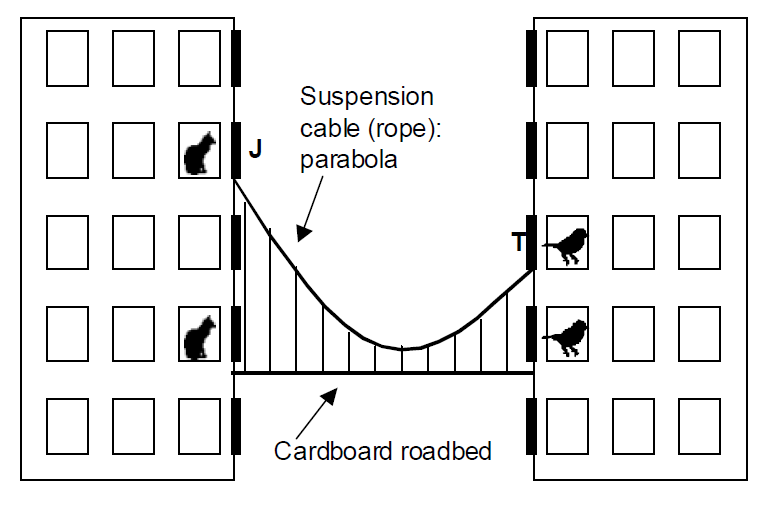
\includegraphics[width=0.7 \textwidth]{2004i.png}
					\caption{} \label{2004i}
				\end{figure}

				\begin{algorithm}[b]
				\caption{}
				\label{2004i}
					\begin{algorithmic}[1]
						\State $Ans  \gets \text{无解}$
						\For{
%							枚举 $i$, 从
							$i = 1$ 到 $ \text{挂绳索的两个楼层中的较低者} - 1$
						}
							\If{两栋房子的第 $i$ 层楼中,一栋有猫,一栋有鸟}
								\State $Ans \gets 3i-2$,并退出循环。 
							\EndIf
							\If{两栋房子的第 $(i + 1)$ 层楼中至少有一栋有猫,第 $i$ 层楼中至少有一栋有鸟}
								\State $Ans \gets 3i-1.5$,并退出循环。 
							\EndIf
						\EndFor
					\end{algorithmic}
				\end{algorithm}	
				
			\subsubsection{算法讨论}
				根据生活经验,绳索越长,平板低,故需要求出平板最低的高度。
%				绳索越长平板越低的结论稍后证明。
				
				通过题目给出的常量,用算法 \ref{2004i} 即可求出此最低高度 $Ans$。
				
				求出高度 $Ans$ 后,就要通过物理手段求绳索的长度了。
				
				{\theorem 线缆呈抛物线形。}
				
				\vskip0.5em

\begin{tabular}{p{.3\textwidth} p{.6\textwidth}}
    \vspace{0pt} 
\centering
\definecolor{cczzqq}{rgb}{0.8,0.6,0}
\definecolor{qqzzff}{rgb}{0,0.6,1}
\begin{tikzpicture}[line cap=round,line join=round,>=stealth',x=1.0cm,y=1.0cm]
\draw[->,color=black] (-0.5,0) -- (3.34,0) node[right] {$x$};
%\foreach \x in {1,2,3}
%\draw[shift={(\x,0)},color=black] (0pt,2pt) -- (0pt,-2pt) node[below] {\footnotesize $\x$};
\draw[->,color=black] (0,-0.5) -- (0,7.75) node[left] {$y$};
%\foreach \y in {-1,1,2,3,4}
%\draw[shift={(0,\y)},color=black] (2pt,0pt) -- (-2pt,0pt) node[left] {\footnotesize $\y$};
\draw[color=black] (0pt,-10pt) node[left] {$O$};
\newcommand{\lenghtlengthiii}{2.5}
\draw [samples=50,rotate around={0:(0,0)},xshift=0cm,yshift=0cm,color=cczzqq,domain=0:\lenghtlengthiii)] plot (\x,{(\x)^2});
\draw [color=qqzzff, -> ] (0,0) -- (-0.8,0) node[above] {$\mathbf{F}$};
\draw [color=qqzzff, -> ] (\lenghtlengthiii,\lenghtlengthiii*\lenghtlengthiii) -- 
		({\lenghtlengthiii + 1.2*sqrt(\lenghtlengthiii*\lenghtlengthiii*4+1)/(\lenghtlengthiii*\lenghtlengthiii*4+1)},
		{\lenghtlengthiii * \lenghtlengthiii + 1.2* 2 * \lenghtlengthiii *sqrt(\lenghtlengthiii*\lenghtlengthiii*4+1)/(\lenghtlengthiii*\lenghtlengthiii*4+1)}) node[above] {$\mathbf{F}_2$};
%\draw[shift={(\lenghtlengthiii,0)},color=black] (0pt,2pt) -- (-0pt,-2pt) 
%		node[below 
%		right
%		] {$x$}
%		;
\fill [color=qqzzff] (0,0) circle (1.5pt);
\fill [color=qqzzff] (\lenghtlengthiii,\lenghtlengthiii*\lenghtlengthiii)  circle (1.5pt)
node[above left,color=black
		] {$P$};

\foreach \x in {1,2,3,4,5}
\draw [color=qqzzff, -> ] (\x * \lenghtlengthiii / 5,\x * \lenghtlengthiii / 5*\x * \lenghtlengthiii / 5 ) -- 
		 (\x * \lenghtlengthiii / 5,0);
\draw [color=qqzzff, below] (\lenghtlengthiii / 2, 0) node {$\mathbf{G} = (0, -\rho x)$};
\end{tikzpicture}
				\captionof{figure}{}
				\label{2004i2}
    & 
    \vspace{0pt}
				\begin{pf}
					如图 \ref{2004i2} 将线缆的最低点平移到原点 $O$。设线缆可表达为函数 $y(x)$。任取另外一点$P(x, y(x))$,分析 $O$ 到 $P$ 的绳索的受力。原点处有一个水平的拉力 $\mathbf{F} = (-F, 0)$,$P(x, y(x))$ 处有一个沿切线方向的力 $\mathbf{F}_2$。
%					绳索处处受力相等,故 $|\mathbf{F}| = |\mathbf{F}_2|$。
					负重的线密度 $\rho$,水平方向的长度 $x$,故总负重 $\mathbf{G} = (0, -\rho x)$。整段绳子动量 $\mathbf{p} \equiv \mathbf{0}$,故
					\begin{align}
						\mathbf{F} + \mathbf{F}_2 + \mathbf{G} = \mathbf{0}
					\end{align}
					即
					\begin{align}
						\begin{cases}
							-F + F_2\cos\theta + 0 = 0\\
							0 +  F_2\sin\theta - \rho x = 0\\
							\tan\theta  = 
%								\left. \mathrm{d} y(x) / \mathrm{d} x \right|_{x}
								\mathrm{d} y(x) / \mathrm{d} x
						\end{cases}
					\end{align}
					整理可得
					\begin{align}
						\frac{\mathrm{d} y(x)}{ \mathrm{d} x} = \tan\theta = \frac{\rho x}{F}
					\end{align}
					分离变量,积分
					\begin{align}
						\int F \mathrm{d} y(x) =  \int \rho x\mathrm{d} x + \mathrm{C}
					\end{align}
					即 
					\begin{align}
						y(x) = \frac{\rho}{2 F} x^2 + \mathrm{C}
					\end{align}
					$\rho / (2 F)$ 为与绳子有关的常数,故命题得证。 
					 \qed
				\end{pf}
\end{tabular}
			令 $\rho / (2 F) = a$。在固定了平板的高度后,也就确定了抛物线的最低点,以及到两个窗户的竖直距离 $h_{1,2}$。接下来需要确定 $a$ 和最低点到两个窗户的水平距离。即求 $a, x_1, x_2$ 满足
			\begin{align}
				ax_1^2 &= h_1 \label{2004iaaa}\\
				ax_2^2 &= h_2 \label{2004ibbb}\\
				x_1 + x_2 &= L \label{2004iccc}
			\end{align}
			其中 $L$ 是
%			两栋
			房屋间的距离。
			$\sqrt{\eqref{2004iaaa}} + \sqrt{\eqref{2004ibbb}}$ 得
			\begin{align}
				\sqrt{a} L& = \sqrt{a}x_1 + \sqrt{a}x_2 = \sqrt{h_1} + \sqrt{h_2}
				\intertext{故}
					a &= \left(\left.\left(\sqrt{h_1} + \sqrt{h_2}\right) \right/ L \right)^2\\
					x_1 &= \sqrt{h_1 / a}\\
					x_2 &= \sqrt{h_2 / a}
			\end{align}
			这样最后的问题就是求曲线 $y = f(x) = ax^2, x \in [-x_1, x_2]$ 的长度 $l$。根据微积分知识,答案应当为
			\begin{align}
				l & =\int_{-x_1}^{x_2} \sqrt{{\mathrm{d} x}^2 + {\mathrm{d} y}^2} \notag \\
					& =\int_{-x_1}^{x_2} \mathrm{d} x \sqrt{1 + {(\mathrm{d} y /\mathrm{d} x)}^2} \notag  \\ 
					& =\int_{-x_1}^{x_2} \sqrt{1 + {(2ax)}^2} \mathrm{d} x \notag  \\ 
					& = \left[ \frac{2 a x \sqrt{4 a^2 x^2+1} + \sinh^{-1}2 a x}{4 a}\right]_{-x_1}^{x_2} \label{2004id}
			\end{align}
			根据 \eqref{2004id} 就可直接求出答案。% 最后是绳索长度与木板高度的单调性证明。
%			{\theorem 绳索越长平板越低。}
			
			\subsubsection{时空复杂度}
				时间复杂度 $\mathcal{O}\left(N\right)$。
					
				空间复杂度 $\mathcal{O}\left(N\right)$。
		\newpage
